% 小时百科图标

\begin{issues}
\issueDraft
\issueOther{需要给出明确参数(自由粒子波函数)}
\end{issues}

小时百科的图标是由 4 条丝带组成 3D 立体图, 从数学上来看, 每条丝带的形状分别是一个高斯分布函数\upref{GausPD}, 物理上, 四条丝带可以分别看作量子力学中自由粒子随时间演化的过程\upref{GausWP}. 艺术上, 可以寓意为海浪. 目前图标分为立体版本(\autoref{xwLogo_fig2} )和扁平化版本(\autoref{xwLogo_fig1} ).

\begin{figure}[ht]
\centering
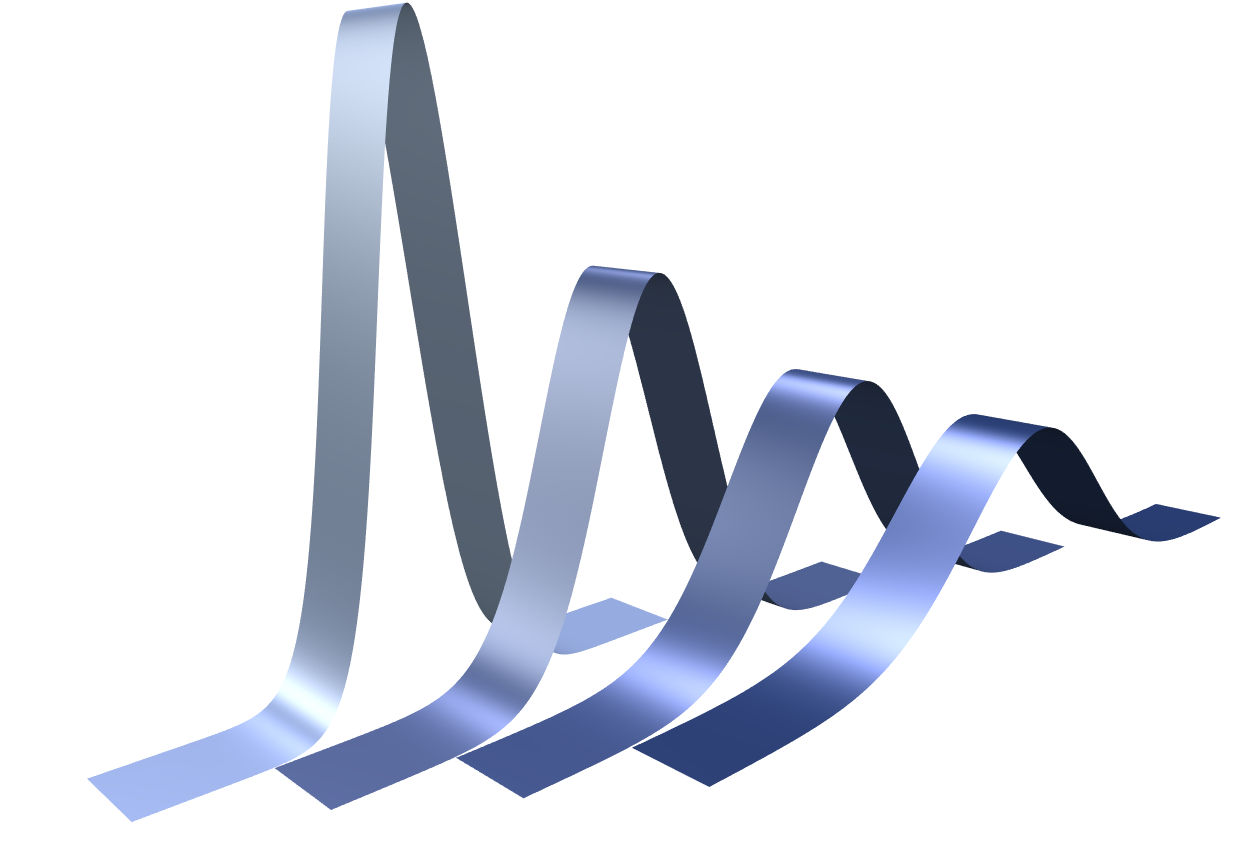
\includegraphics[width=8.3cm]{./figures/xwLogo_2.png}
\caption{立体图标, 完成于 2014 年 10 月} \label{xwLogo_fig2}
\end{figure}

\begin{figure}[ht]
\centering

\includegraphics[width=8cm]{./figures/xwLogo_1.pdf}
\caption{扁平化图标, 完成于 2020 年 9 月} \label{xwLogo_fig1}
\end{figure}
